\documentclass[compress]{beamer}


% Try the class options [notes], [notes=only], [trans], [handout],
% [red], [compress], [draft], [class=article] and see what happens!

% For a green structure color use:
\colorlet{structure}{green!50!black}

\mode<article> % only for the article version
{
  \usepackage{beamerbasearticle}
  \usepackage{fullpage}
  \usepackage{hyperref}
}



\beamertemplateshadingbackground{red!10}{blue!10}

%\setbeamertemplate{footline}[page number]
%\usepackage{beamerthemeshadow}

\usepackage{pgf,pgfarrows,pgfnodes,pgfautomata,pgfheaps,pgfshade}
\usepackage{graphicx}
\usepackage{amsmath,amssymb}
\usepackage[latin1]{inputenc}
\usepackage{colortbl}
\usepackage[english]{babel}


%\usepackage{times}

% Use some nice templates
\beamertemplatetransparentcovereddynamic

% own commands

\newcommand{\be}{\begin{equation}}
\newcommand{\ee}{\end{equation}}
\newcommand{\bra}[1]{\left\langle #1 \right|}
\newcommand{\ket}[1]{\left| #1 \right\rangle}
\newcommand{\braket}[2]{\left\langle #1 \right| #2 \right\rangle}
\newcommand{\element}[3]{\bra{#1}#2\ket{#3}}
\newcommand{\normord}[1]{\left\{#1\right\}}
\newcommand{\OP}[1]{{\bf\widehat{#1}}}
%\newcommand{\OP}[1]{{\bf\widehat{#1}}}
\newcommand{\Hd}{\hat{H}^{\rm d}}
\newcommand{\Ho}{\hat{H}^{\rm od}}
\newcommand{\matr}[1]{{\bf \cal{#1}}}
\def\d{\text{d}}
\def\sech{\text{sech}}
\def\Cdot{\!\cdot\!} 
\def\e{\text{e}}
\def\L_2{\L_{2}}
\def\fm{\:\:\mathrm{fm}^{-1}}

%\newcommand{\braket}[1]{\langle#1\rangle}
%\newcommand{\Span}{\OPeratorname{sp}}
%\newcommand{\tr}{\OPeratorname{trace}}
%\newcommand{\diag}{\OPeratorname{diag}}

\newcommand{\pdiff}[2]{\frac{\partial#1}{\partial#2}}
\newcommand{\wedgeprod}[2]{\overset{#2}{\underset{#1}{\wedge}}}
\newcommand{\directsum}[2]{\overset{#2}{\underset{#1}{\bigoplus}}}
\newcommand{\Span}{\OPeratorname{span}}
\newcommand{\Hilb}{{\mathcal{H}}}
\newcommand{\Proj}{{\mathcal{P}}}
\newcommand{\Model}{{\mathcal{M}}}
\newcommand{\CalS}{{\mathcal{S}}}
\newcommand{\PhiFD}{\Phi^\mathrm{FD}}
\newcommand{\Ind}{{\mathcal{I}}}
\newcommand{\rmd}{\mathrm{d}}
\newcommand{\sgn}{\OPeratorname{sgn}}
\newcommand{\eofproof}{\hspace{1em}$\diamondsuit$}

%\usetheme{}
%\useinnertheme{rectangle}
\title[MSU January 5, 2011]{Living on the edge of stability, challenges to nuclear theory in the FRIB era}

\author[OSU, March 1, 2012]{%
Kevin Fossez, Morten Hjorth-Jensen, Thomas Papenbrock and Ragnar Stroberg}
\institute[ORNL, MSU, FRIB etc]{MSU, NSCL/FRIB, ORNL and UTK, Reed College, University of Washington}


\date[July sand August  2018]{Nuclear Talent course 2018, Xinxiang, Henan Normal University}

\begin{document}

\frame{\titlepage}

%\section<presentation>*{Outline}

%\frame
%{
%  \frametitle{Outline}
%  \tableofcontents[part=1,pausesections]
%  \tableofcontents[part=1]
%}

%\AtBeginSubsection[]
%{
%  \frame<handout:0>
%  {
%    \frametitle{Outline}
%    \tableofcontents[current,currentsubsection]
%  }
%}

\part<presentation>{Main Talk}


%\frame{\titlepage}

%\frame{\tableofcontents}

%\part<presentation>{Main Talk}

\frame
{
  \frametitle{ }
%     \vspace{-3cm}
      \begin{figure}[htp]
        \centering	
        	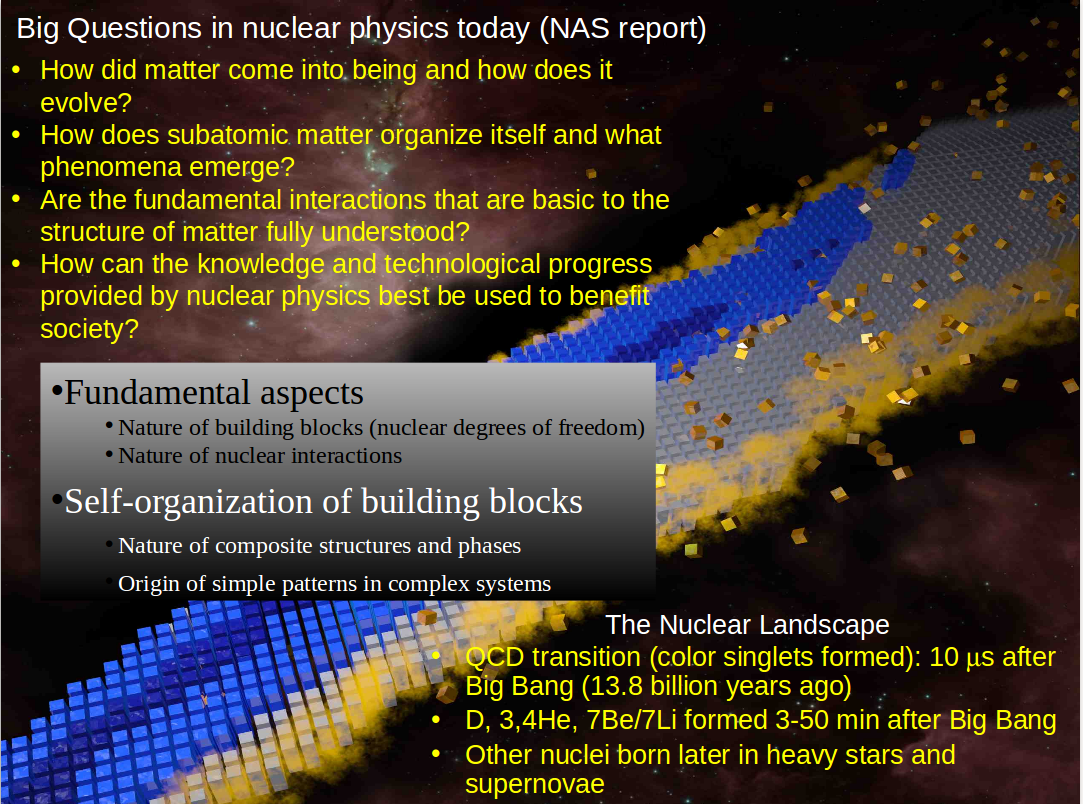
\includegraphics[width=1.0\textwidth]{Figures/bigquestions.png}
      \end{figure}
}


\frame
{
  \frametitle{Many-body theories 2005, Barrett, Dean, MHJ, Vary, 2004, JPG {\bf 31}}
It is our firm belief 
that new developments in many-body theories
for nuclear problems should contain as many as possible of the 
following ingredients:
\begin{itemize}
\item
It should be fully microscopic and start with present two- and three-body
interactions derived from {\it e.g.,} effective field theory;
\item It can be improved upon systematically, e.g., by inclusion of
three-body interactions and more complicated correlations;
\item It allows for description of both closed-shell 
systems and valence systems;
\item For nuclear systems where shell-model studies are the only feasible ones,
viz., a small model space requiring an effective interaction, 
one should be able to
derive  effective two and three-body 
equations and interactions for the shell
model;
\end{itemize}

}



\frame
{
  \frametitle{Many-body theories 2005, Barrett, Dean, MHJ, Vary, 2004, JPG {\bf 31}}
\begin{itemize}
\item It is amenable to parallel computing;
\item It can be used to generate excited spectra for nuclei like 
where many shells are involved (It is hard for the traditional shell model
to go beyond one major shell.  The inclusion of several shells may imply 
the need of  complex effective interactions
needed in studies of weakly bound systems); and
\item Finally, nuclear structure results should be used in marrying microscopic 
many-body results with reaction studies. This will be another hot topic
of future {\it ab initio} research.
\end{itemize}

{\bf Most of these topics are nowadays standard ingredients in most many-body methods}

}





\frame
{
  \frametitle{Many-body theories 2005}
%     \vspace{-3cm}
      \begin{figure}[htp]
        \centering	
        	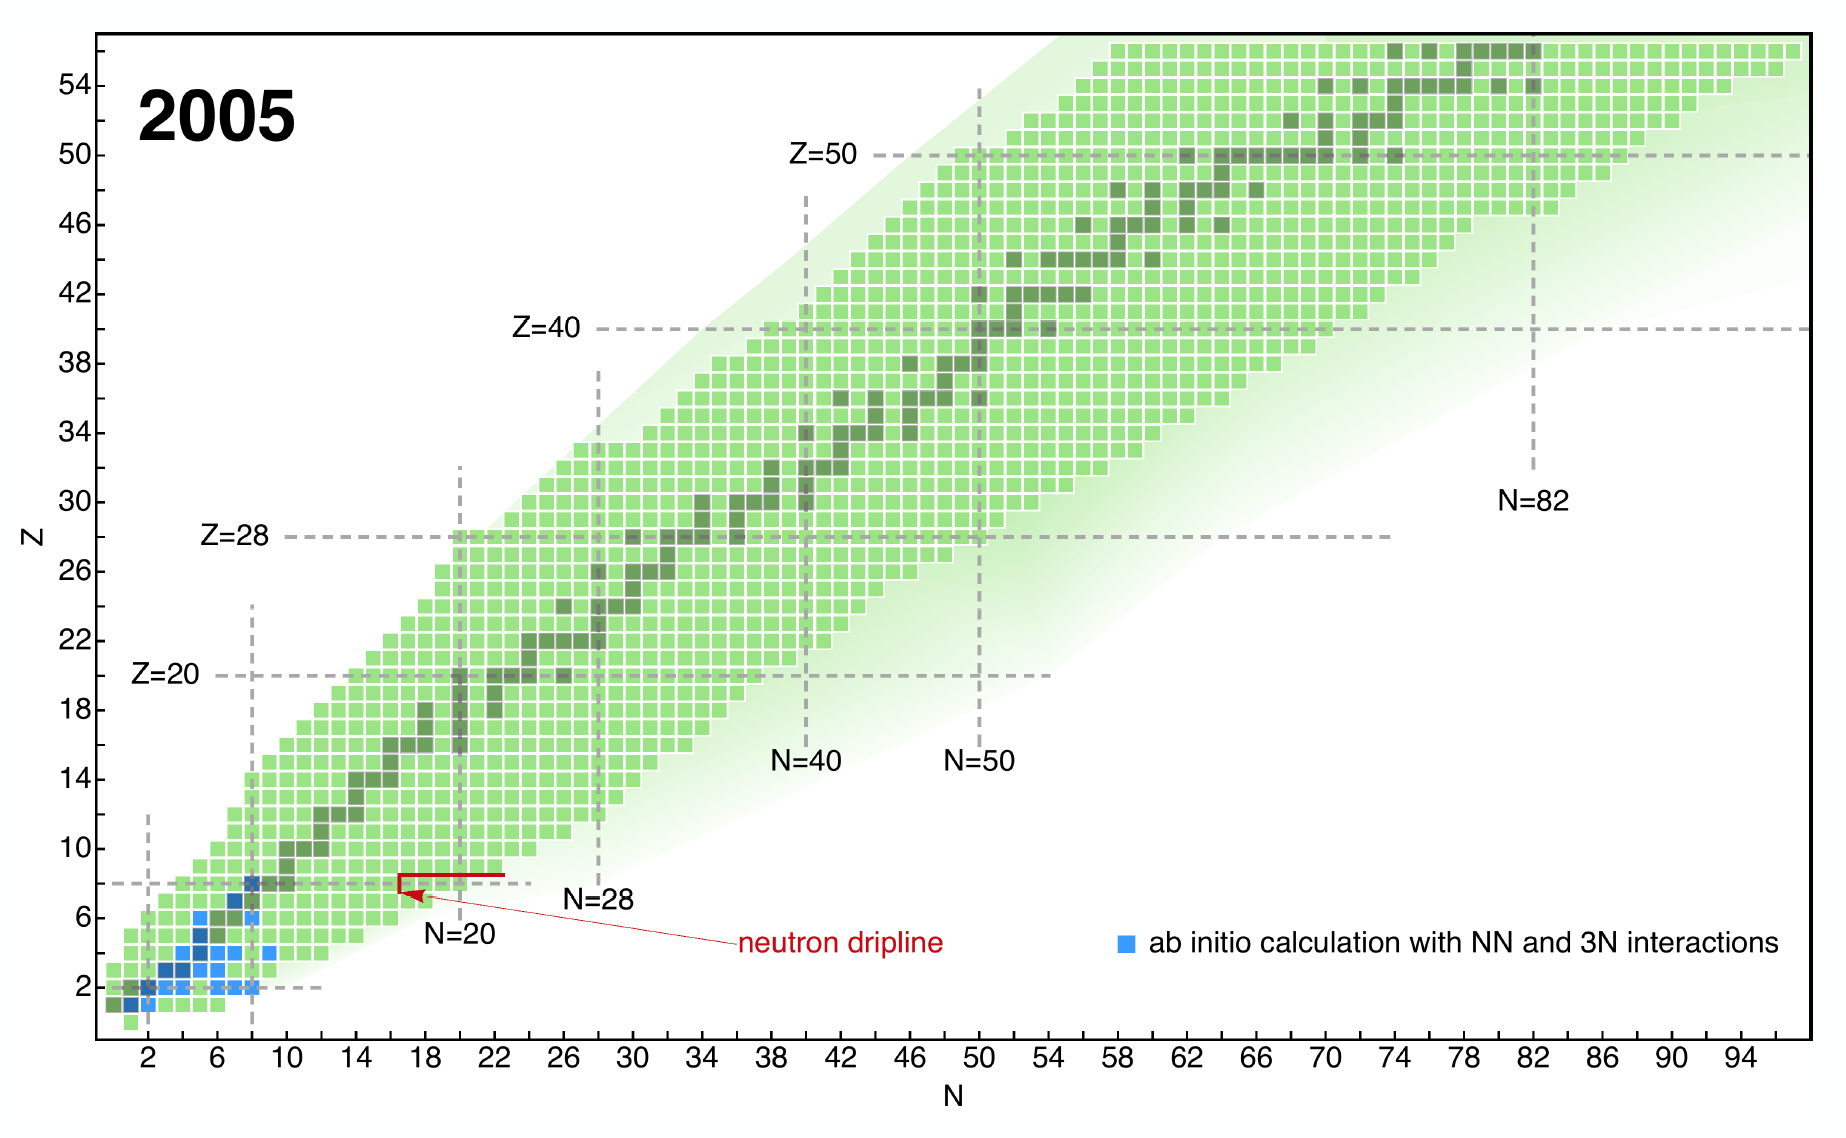
\includegraphics[width=1.1\textwidth]{Figures/abinitio2005.png}
      \end{figure}
}

\frame
{
  \frametitle{In 2015 }
%     \vspace{-3cm}
      \begin{figure}[htp]
        \centering	
        	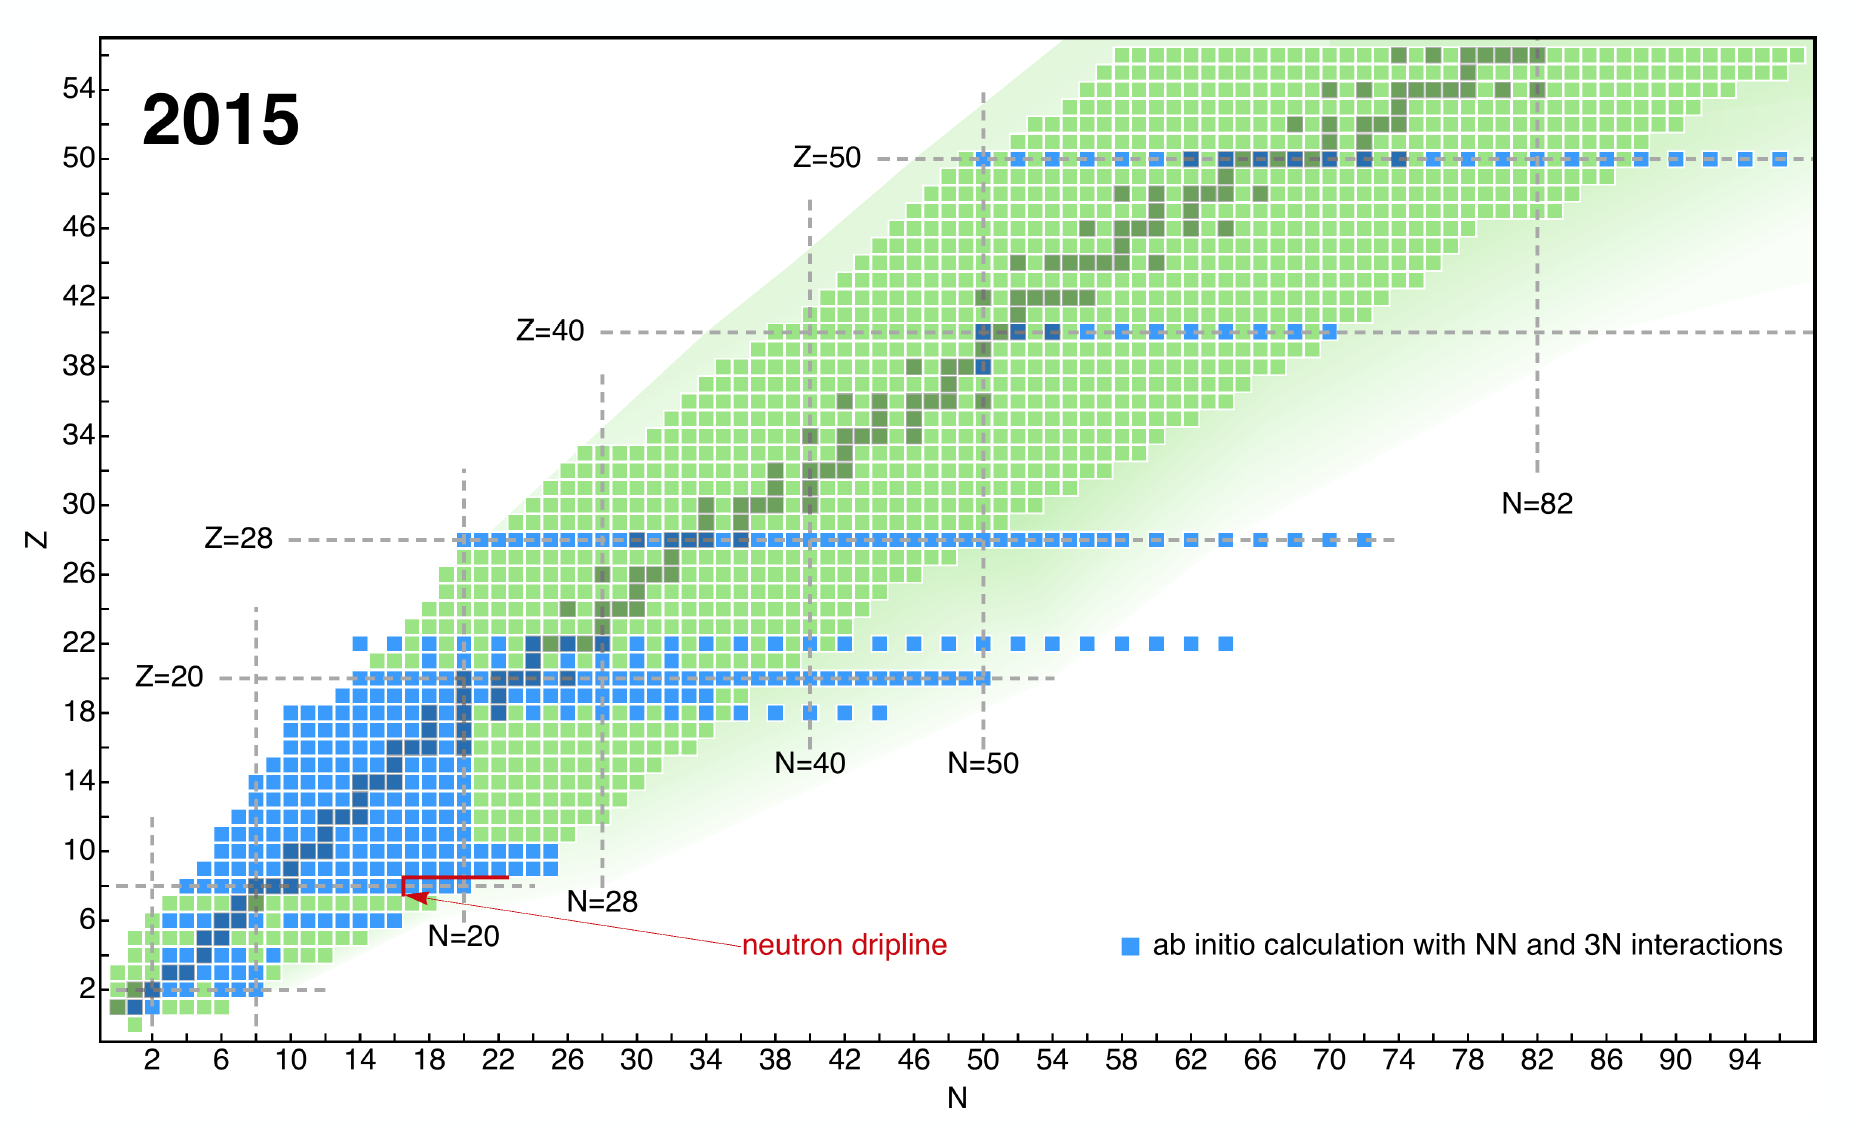
\includegraphics[width=1.1\textwidth]{Figures/abinitio2015.png}
      \end{figure}
}

\frame
{
  \frametitle{And in 2018 (not complete) }
%     \vspace{-3cm}
      \begin{figure}[htp]
        \centering	
        	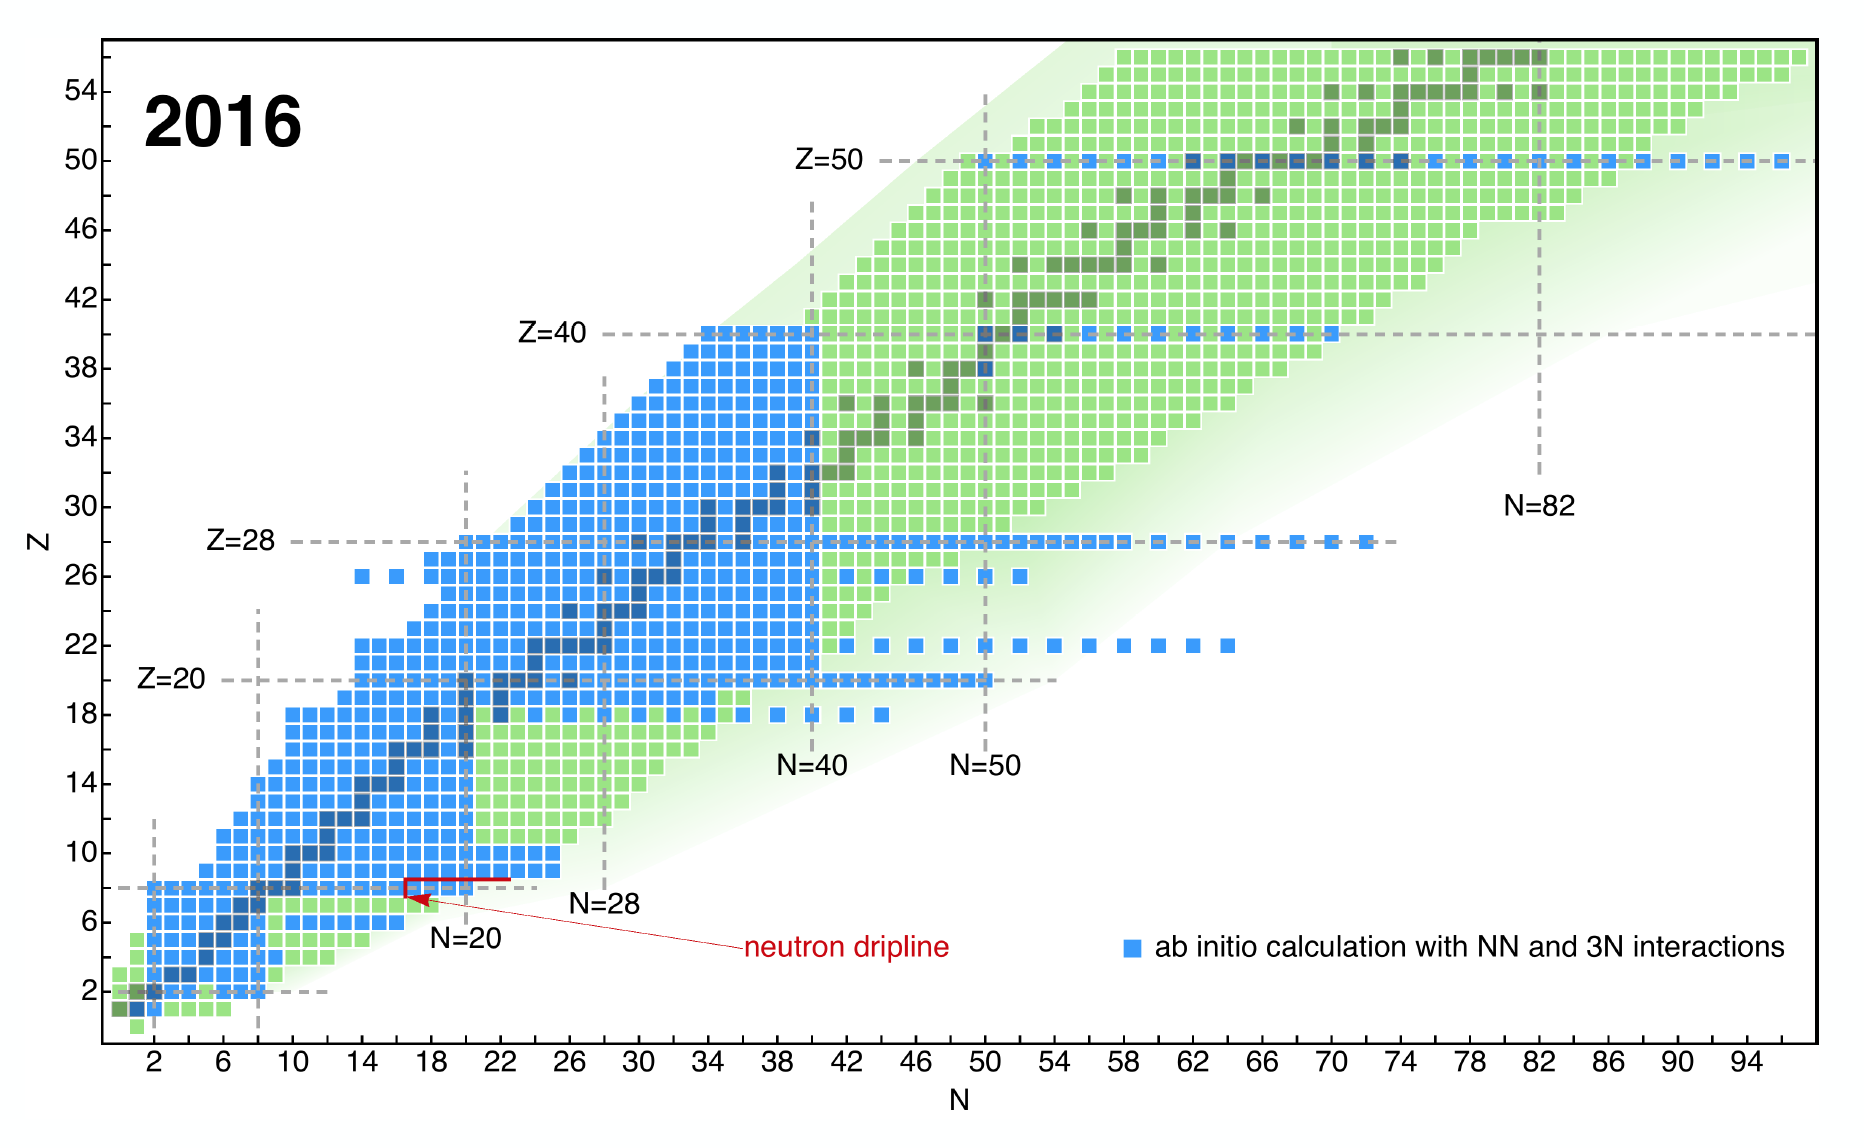
\includegraphics[width=1.1\textwidth]{Figures/abinitio2016.png}
      \end{figure}
}

\frame
{
  \frametitle{Huge progress in many-body theories }
\begin{itemize}
\item Lattice QCD and lattice effective field theory
\item FCI quantum Monte Carlo
\item Full configuration interaction theory (Shell Model and Variants)
\item In-Medium Similarity Renormalization Group
\item Coupled Cluster theory
\item Self-Consistent Green's Functions
\item Various Monte Carlo methods
\item Density functional theories
\item Now and the future: quantum computing and machine learning
\item And several other approaches
\end{itemize}
}



\frame
    {
      \frametitle{Important questions from QCD to the nuclear many-body problem}
	
      \begin{footnotesize}
     \begin{columns}
      \column{5.0cm}
\begin{itemize}
\item How to derive the in medium nucleon-nucleon interaction from basic principles?
\item How does the nuclear force depend on the proton-to-neutron ratio?
\item What are the limits for the existence of nuclei?
\item How can collective phenomena be explained from individual motion?
\item Shape transitions in nuclei?
\end{itemize}
The many scales pose a severe challenge to {\em ab initio} descriptions of nuclear systems.
\column{5cm}
      \begin{center}
	%\includegraphics[width=6cm, height=4.5cm]{int_contour2.pdf}
	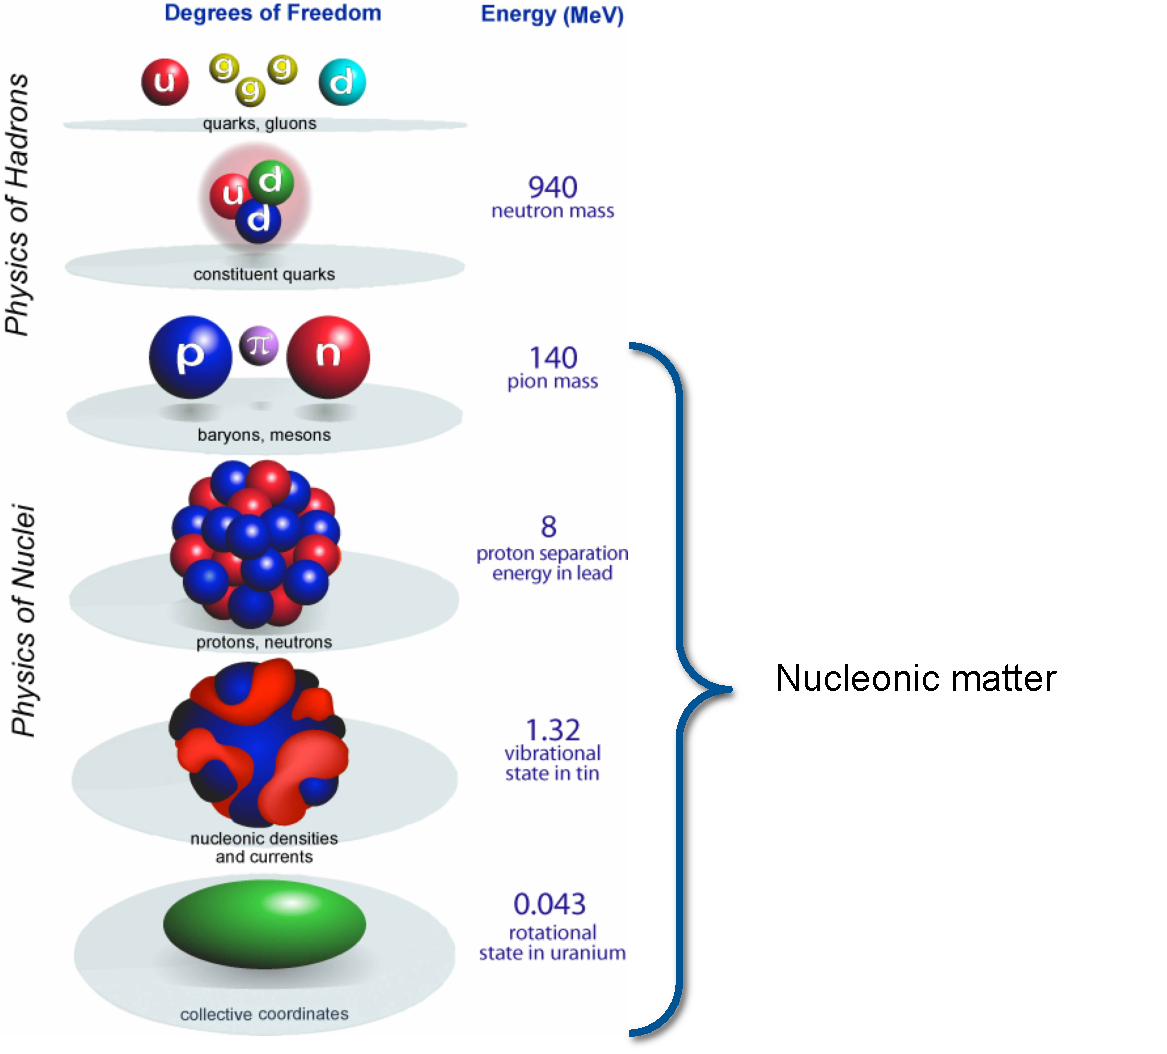
\includegraphics[width=1.3\textwidth]{Figures/witek8.pdf}
      \end{center}
\end{columns}
      \end{footnotesize}
    }





\frame
{
  \frametitle{Consistency between many-body theories (Courtesy of Heiko Hergert@MSU)}
%     \vspace{-3cm}
      \begin{figure}[htp]
        \centering	
        	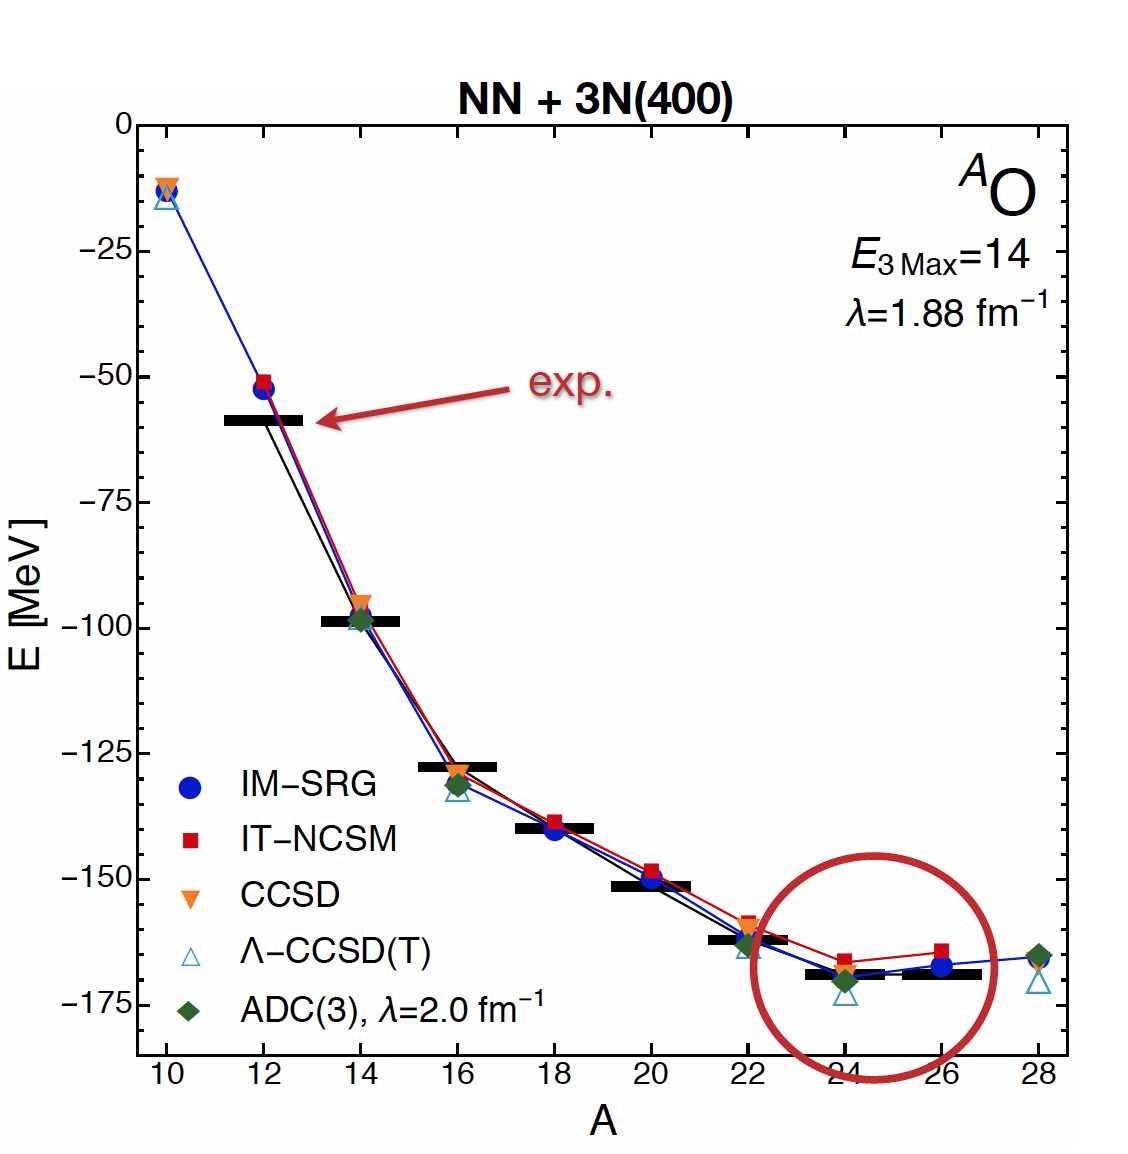
\includegraphics[width=0.7\textwidth]{Figures/consistency.png}
      \end{figure}
}


\frame
{
  \frametitle{Neutron matter calculations with simple Minnesota model for the force, Lecture Notes in Physics {\bf 936} (2017)}
%     \vspace{-3cm}
      \begin{figure}[htp]
        \centering	
        	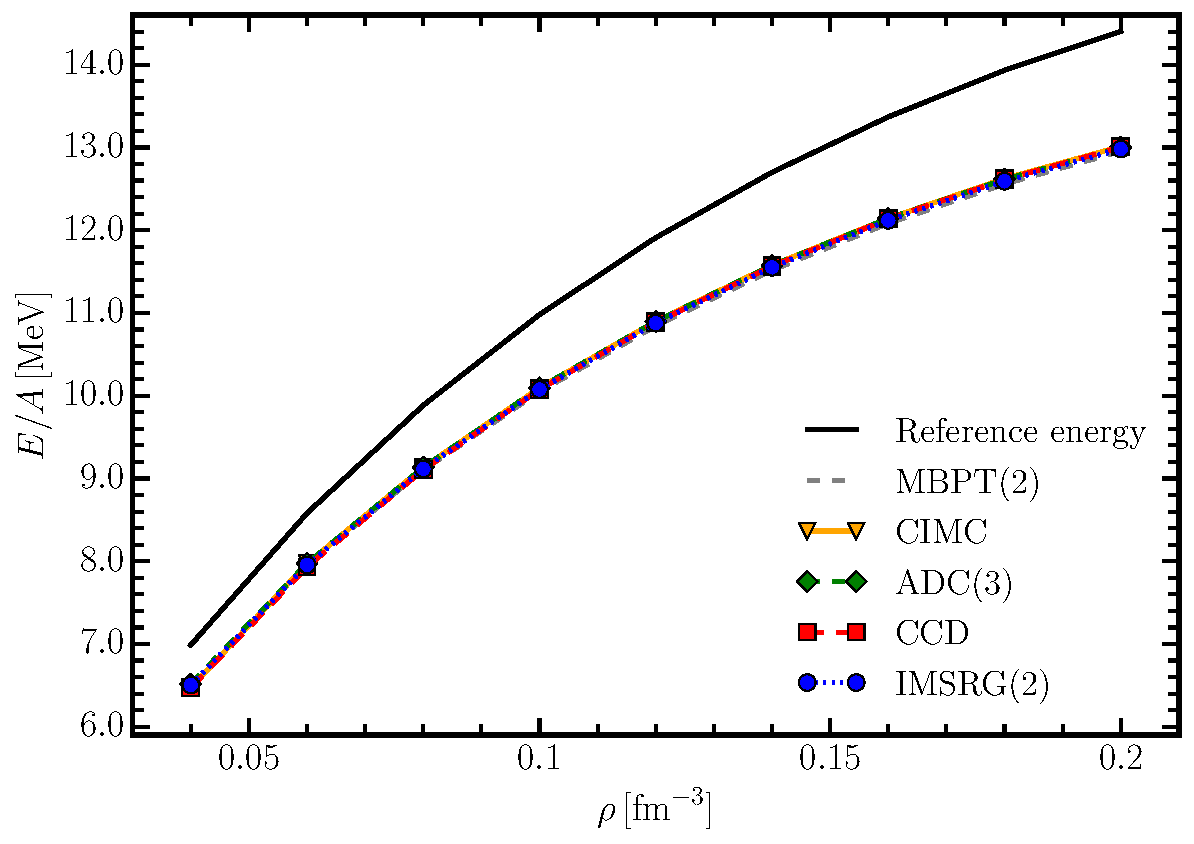
\includegraphics[width=1.0\textwidth]{Figures/imsrg_pnm.pdf}
      \end{figure}
}

\frame
{
  \frametitle{Neutron matter correlation energy, Lecture Notes in Physics {\bf 936} (2017)}
%     \vspace{-3cm}
      \begin{figure}[htp]
        \centering	
        	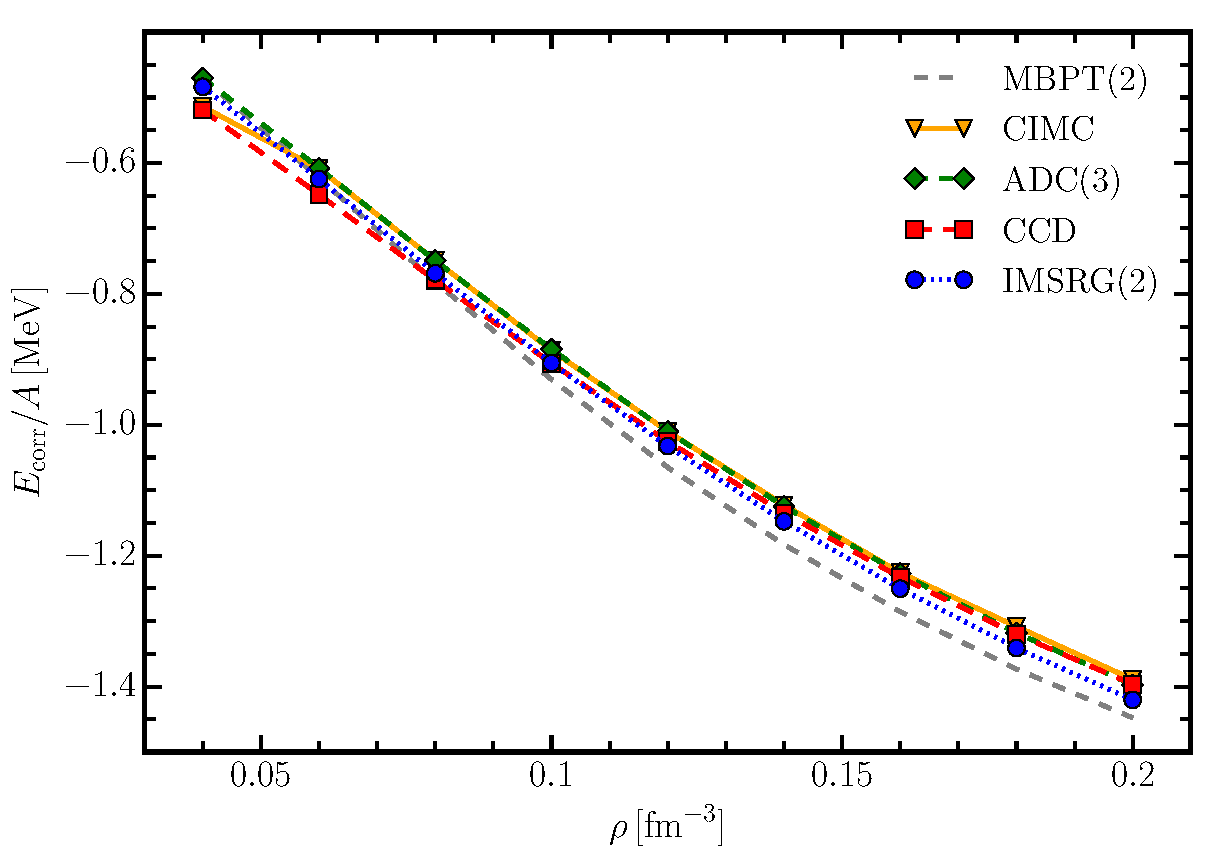
\includegraphics[width=1.0\textwidth]{Figures/imsrg_pnm_ecorr.pdf}
      \end{figure}
}






\frame
{
  \frametitle{Halo nuclei and moving towards the limits of nuclear stability}
  \begin{footnotesize}
   
    \begin{columns}
      \column{4.3cm}
      
      \begin{block}{}
	{\usebeamercolor[fg]{alerted text}{Open Quantum System}}. \\
	Coupling with continuum needs to be taken into account. 
      \end{block}

      \column{4.3cm}
      \begin{block}{}
	{\usebeamercolor[fg]{alerted text}{Closed Quantum System.}}\\ 
	No coupling with external continuum. 
      \end{block}
    \end{columns}
  
  \begin{figure}[htp]
    \centering
    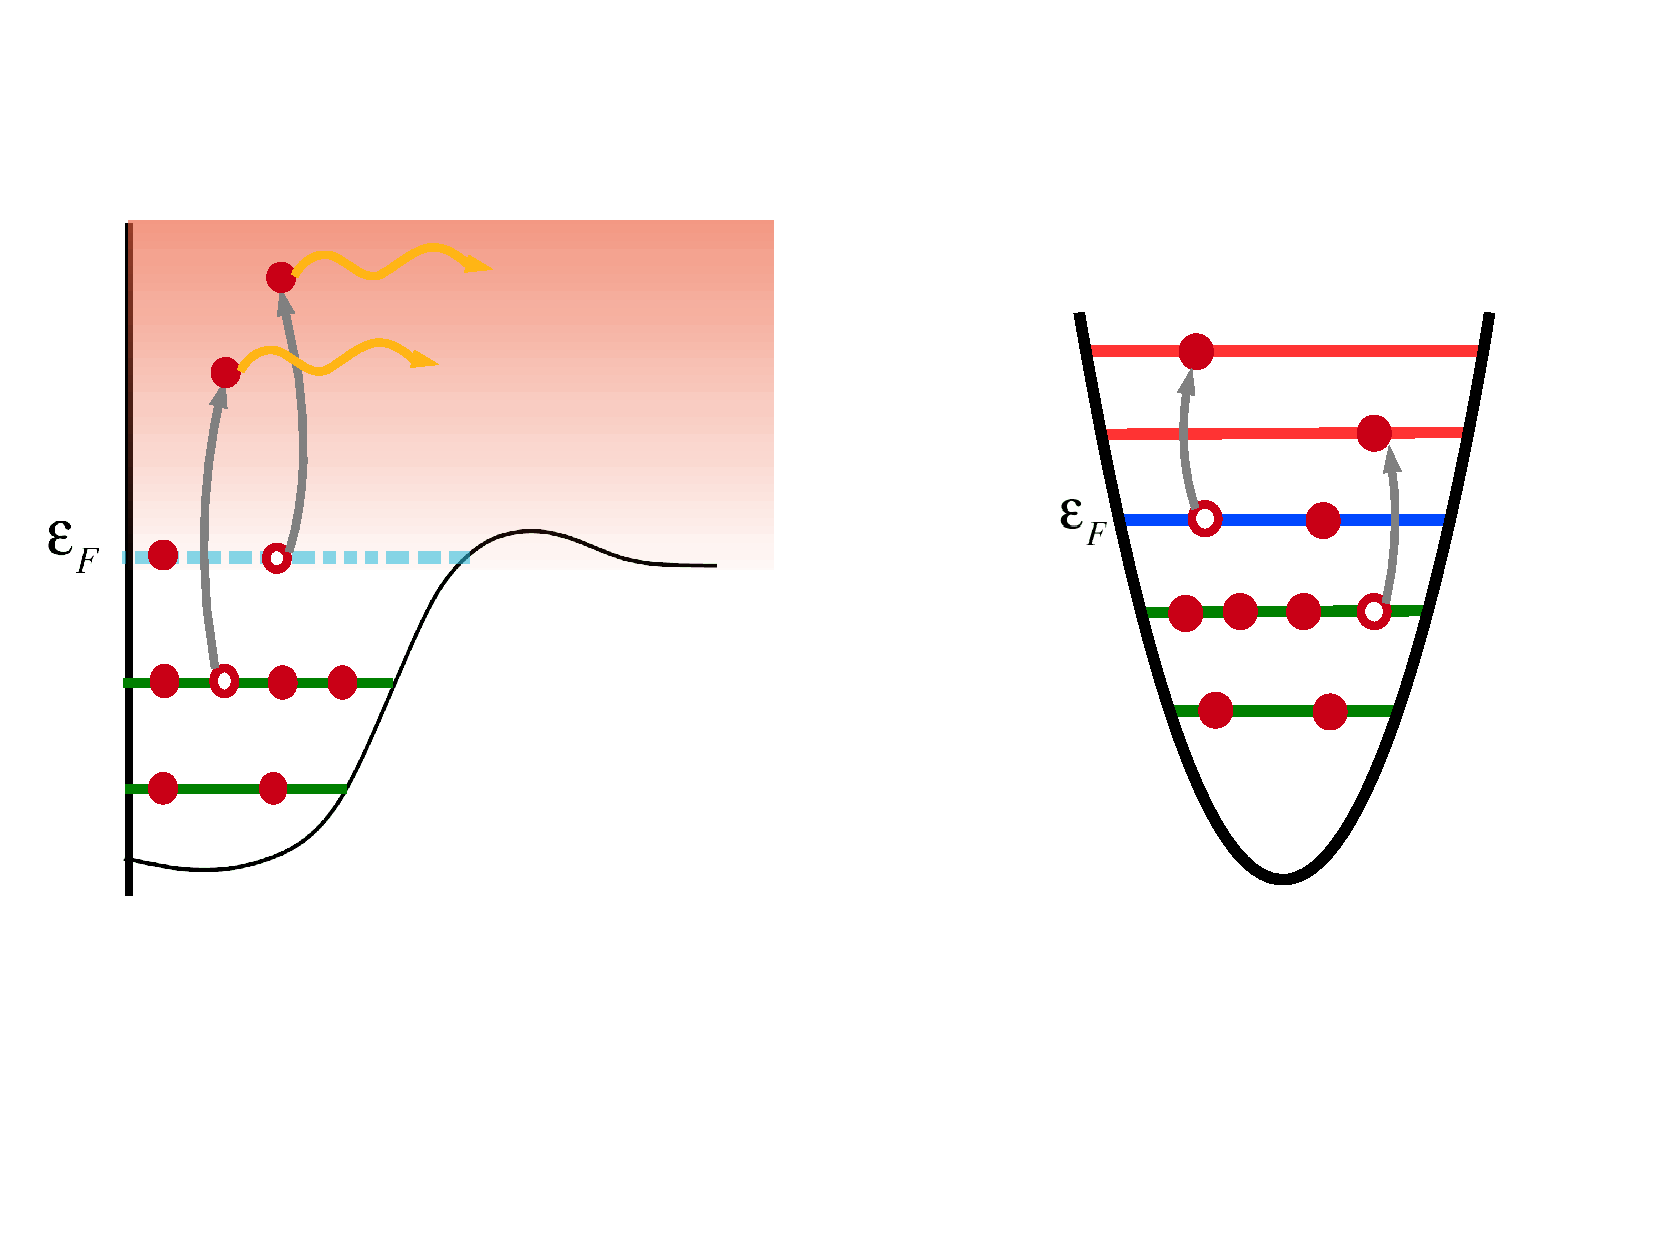
\includegraphics[width=0.8\textwidth]{Figures/fermisurface_unbound.pdf}
  \end{figure}
  
\end{footnotesize}
}


\frame
{
  \frametitle{Shape coexistence and transitions, a multiscale challenge}

  \begin{footnotesize}
    \scriptsize{
    \begin{columns}
      \column{9.5cm}
      \begin{figure}[htp]
        \centering
        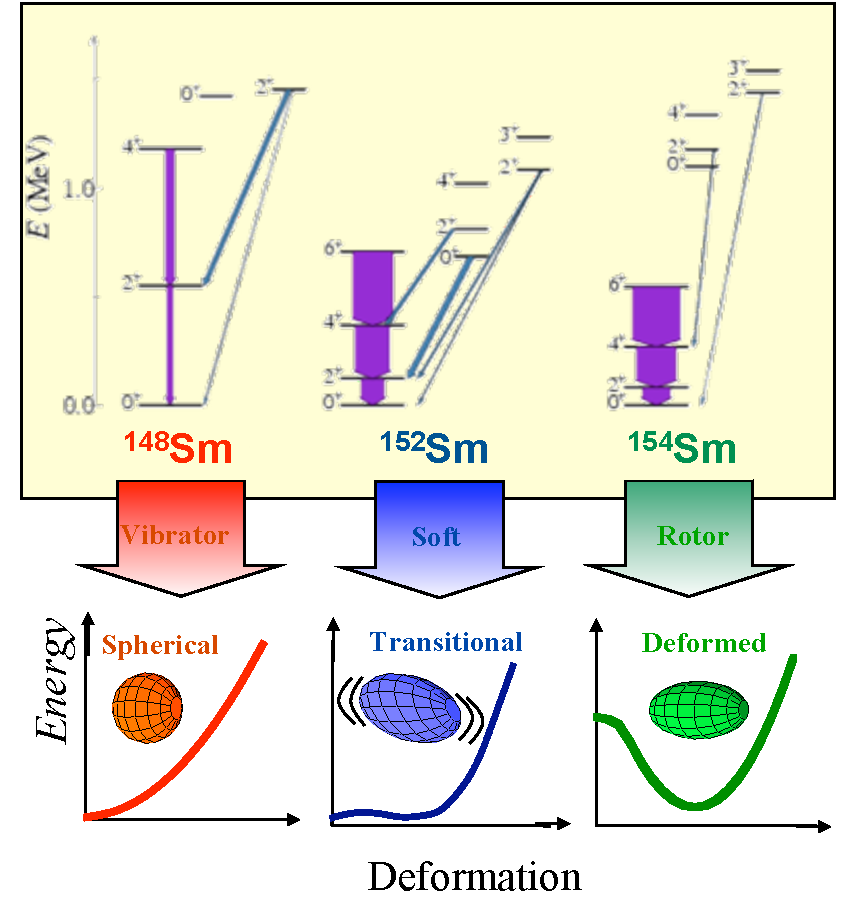
\includegraphics[width=0.75\textwidth]{Figures/witek6.pdf}
      \end{figure}


      \column{3.0cm}
      \begin{block}{Challenges for theory}
        \begin{itemize}
         \item Possible shape transitions, huge spaces needed to describe properly.
         \item Theory: need to marry {\em ab initio} methods with density functional theories in order to describe such systems 
         \item Need a large wealth of experimental data to constrain theory
         \end{itemize}
      \end{block}

    \end{columns}

    }
  \end{footnotesize}
}



\frame
{
  \frametitle{The many interesting intersections}
%     \vspace{-3cm}
      \begin{figure}[htp]
        \centering	
        	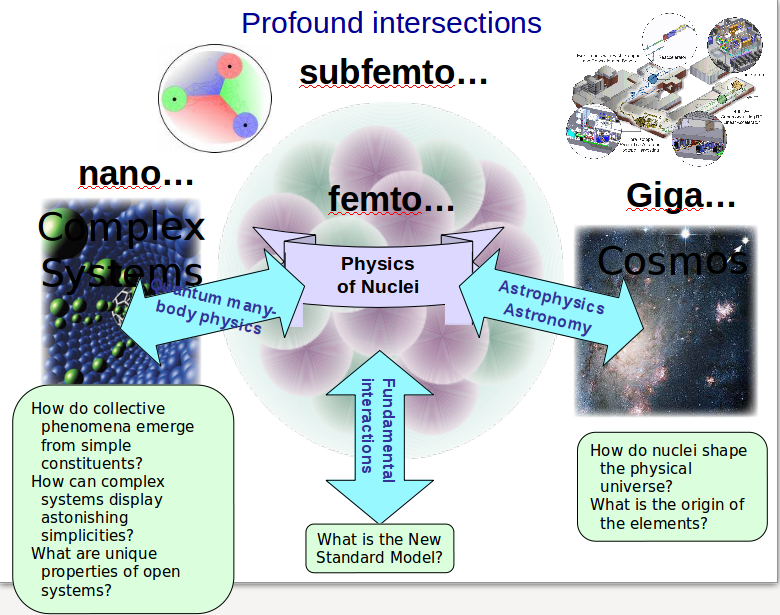
\includegraphics[width=1.0\textwidth]{Figures/crossfield.png}
      \end{figure}
}



\frame
    {
      \frametitle{Known nuclei and predictions}
      \begin{center}
	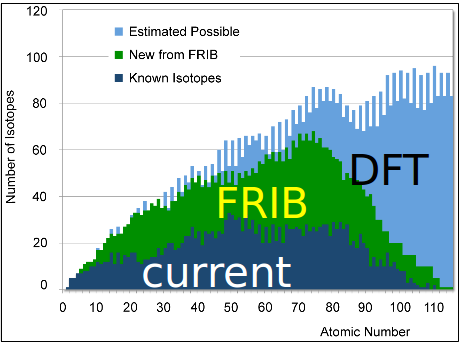
\includegraphics[width=1.0\textwidth]{Figures/current.png}
      \end{center}
    }



\frame
    {
      \frametitle{Do we understand the physics of dripline systems?}
      \begin{footnotesize}
     \begin{columns}
      \column{5.0cm}
\begin{itemize}
\item The oxygen isotopes are the heaviest isotopes for
which the drip line is well established.
\item Two out of four
stable even-even isotopes exhibit a doubly magic nature,
namely $^{22}$O ($Z=8$, $N=14$) and $^{24}$O ($Z=8$, $N=16$).
\item 
The structure of $^{22}$O and $^{24}$O is assumed to be governed
by the evolution of the $1s_{1/2}$ and $0d_{5/2}$  one-quasiparticle states.
\item The isotopes
$^{25}$O
$^{26}$O, $^{27}$O and $^{28}$O are outside the drip line, since the $0d_{3/2}$ orbit is not bound.
\end{itemize}
\column{5cm}
      \begin{center}
	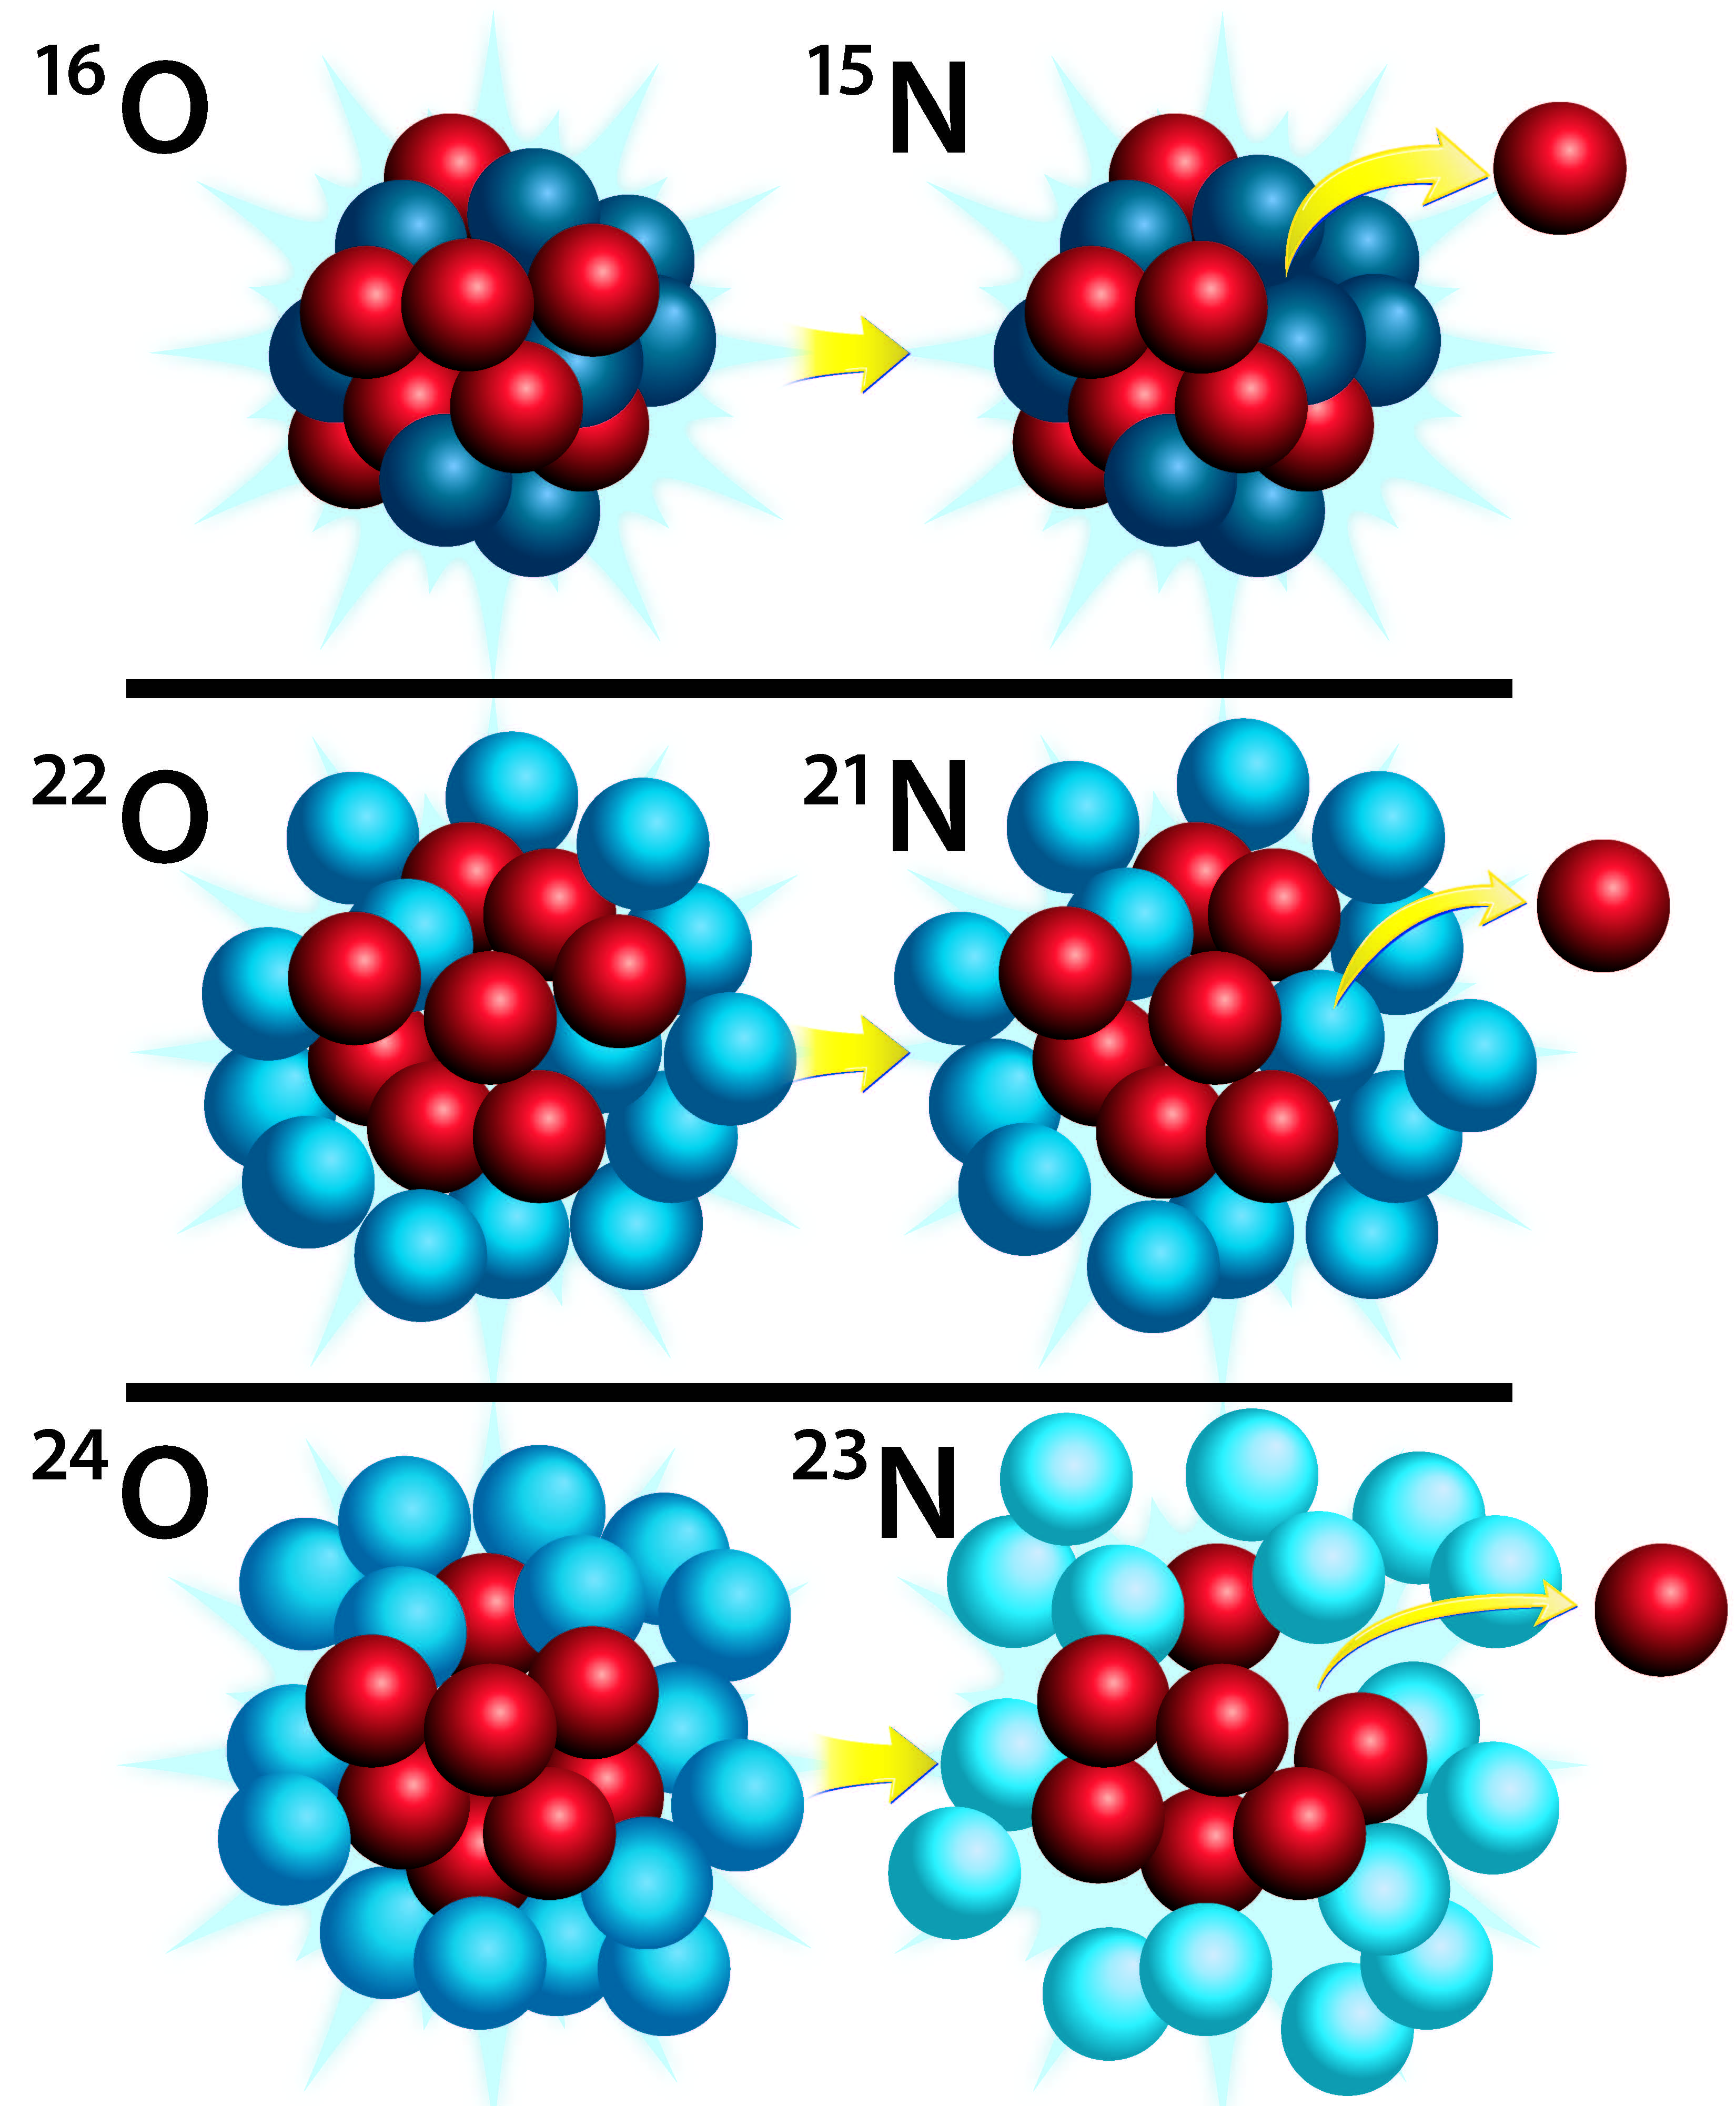
\includegraphics[width=1.2\textwidth]{Figures/oxygens.jpg}
      \end{center}
\end{columns}
      \end{footnotesize}
    }


\frame
    {
      \frametitle{Calcium isotopes and FRIB plans and capabilities}
      \begin{footnotesize}
     \begin{columns}
      \column{5.0cm}
\begin{itemize}
\item The Ca  isotope exhibit several possible closed-shell nuclei $^{40}$Ca, $^{48}$Ca, $^{52}$Ca, $^{54}$Ca,
and  $^{60}$Ca. 
\item  Magic neutron numbers are then $N=20, 28, 32, 34, 40$. 
\item Masses available up to $^{54}$Ca, Gallant {\em et al.},Phys.~Rev.~Lett.~{\bf 109}, 032506 (2012) and K.~Baum {\em et al}, Nature {\bf 498}, 346 (2013).
\item Heaviest observed $^{60}$Ca. NSCL experiment,  O.~B.~Tarasov {\it et al.}, Phys.~Rev.~Lett.~{\bf 121}, 022501 (2018).
\item Which degrees of freedom prevail close to $^{60}$Ca?
\end{itemize}
\column{6cm}
      \begin{center}
	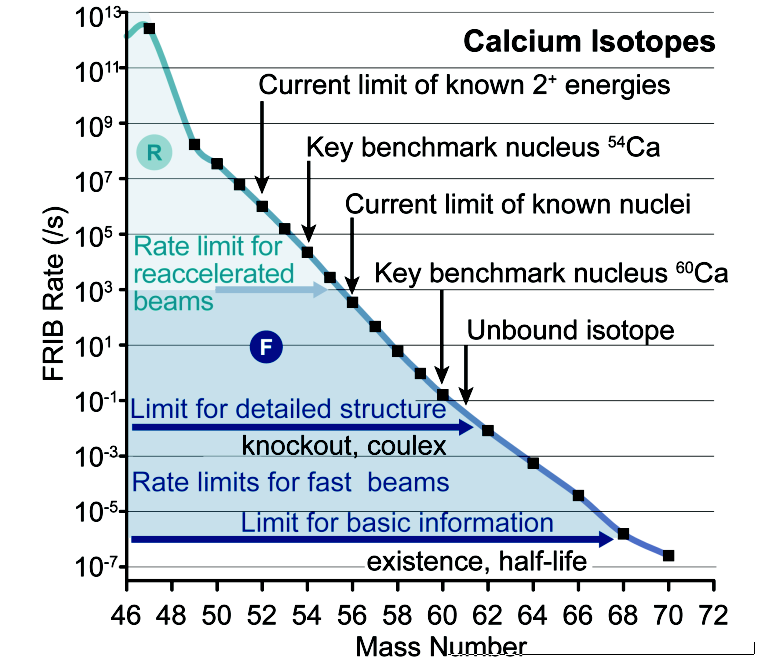
\includegraphics[width=1.15\textwidth]{Figures/careach.png}
      \end{center}
\end{columns}
      \end{footnotesize}
    }




\frame
{
  \frametitle{More on Calcium Isotopes}
      \begin{footnotesize}
     \begin{columns}
      \column{5.0cm}
\begin{itemize}
\item {\bf Mass models and mean field models predict the dripline at $A\sim 70$!} Important consequences for modeling of nucleosynthesis related processes.
\item Can we predict reliably which is the last stable calcium isotope? 
\item And how
does this compare with popular mass models on the market? 
\item And which parts of the underlying forces
are driving the physics towards the dripline?
\end{itemize}
\column{6cm}
\vspace{-3cm}
      \begin{center}
	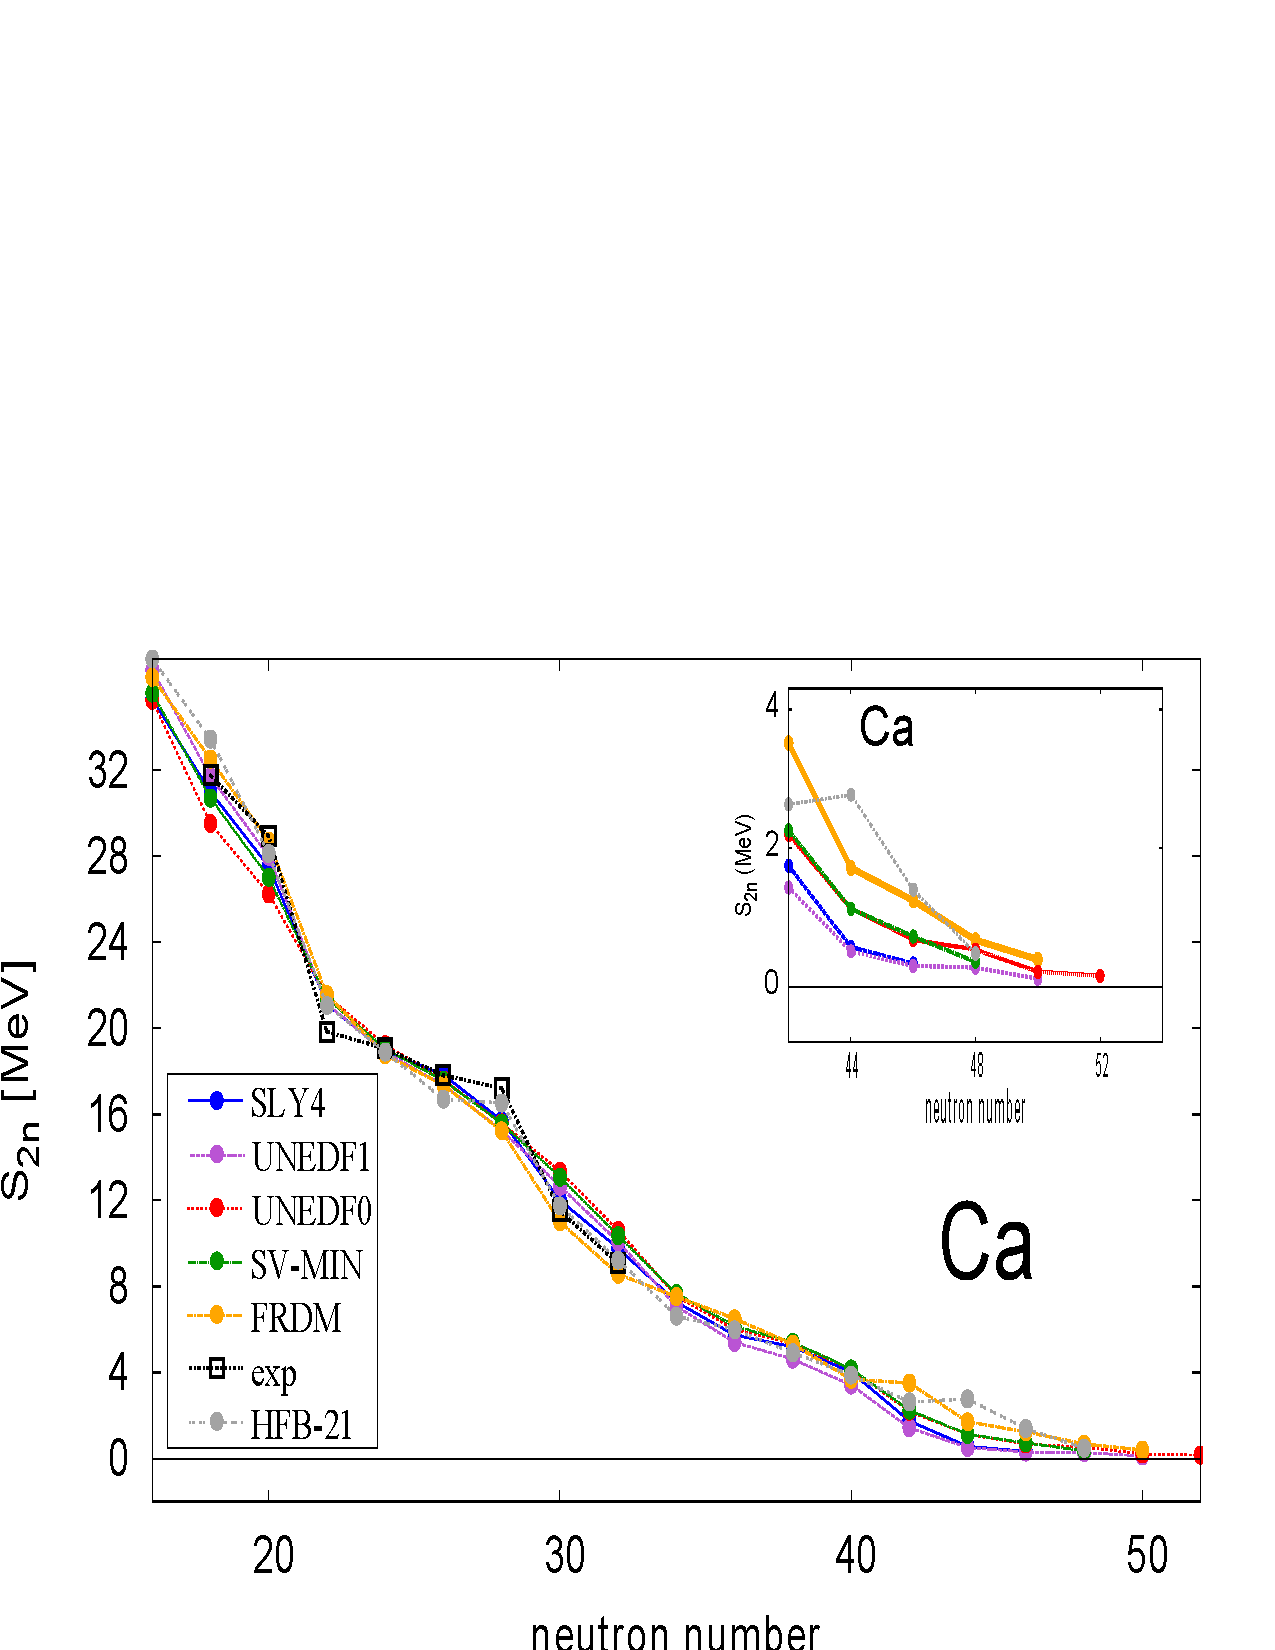
\includegraphics[width=1.15\textwidth]{Figures/witeknatureca.pdf}
      \end{center}
\end{columns}
      \end{footnotesize}
}



\frame
    {
      \frametitle{Other chains of isotopes of crucial interest for FRIB like physics: nickel isotopes}
      \begin{footnotesize}
     \begin{columns}
      \column{5.0cm}
\begin{itemize}
\item This chain of isotopes exhibits four possible closed-shell nuclei $^{48}$Ni, $^{56}$Ni, $^{68}$Ni
and  $^{78}$Ni.  {\bf FRIB plans systematic studies from $^{48}$Ni to $^{88}$Ni.}
\item  Neutron skin possible for $^{84}$Ni at FRIB.
\item Which is the best closed-shell nucleus?
And again, which part of the nuclear forces drives it?  Is it the strong spin-orbit force, the tensor force, or ..?
\end{itemize}
\column{5cm}
      \begin{center}
\setlength{\unitlength}{0.3cm}
\begin{picture}(16,20)
\thicklines
   \put(1,0.5){\makebox(0,0)[bl]{
              \put(0,1){\line(0,1){8}}
              \put(0,9){\line(1,0){8}}
              \put(8,9){\line(0,1){9}}
              \put(8,18){\line(1,0){9}}
              \put(17,1){\line(0,1){17}}
\thinlines
              \put(0.5,2){\line(1,0){7}}
              \put(0.5,4){\line(1,0){7}}
              \put(0.5,6){\line(1,0){7}}
              \put(9.5,6){\line(1,0){7}}
              \put(9.5,8){\line(1,0){7}}
              \put(0.5,12){\line(1,0){7}}
              \put(0.5,8){\line(1,0){7}}
              \put(9.5,4){\line(1,0){7}}
              \put(9.5,2){\line(1,0){7}}
\color{green}
\put(-0.5,11){\makebox(0,0){$1p0f_{5/2}0g_{9/2}$}}
\put(-2,8){\makebox(0,0){$0f_{7/2}$}}
\put(-2,6){\makebox(0,0){$1s0d$}}
\put(-2,4){\makebox(0,0){$0p$}}
\put(-2,2){\makebox(0,0){$0s$}}

\color{red}
\put(3,19){\makebox(0,0){$\pi$--protons}}
\put(3,2){\circle*{0.3}}
\put(5,2){\circle*{0.3}}
\put(1.5,4){\circle*{0.3}}
\put(2.5,4){\circle*{0.3}}
\put(3.5,4){\circle*{0.3}}
\put(4.5,4){\circle*{0.3}}
\put(5.5,4){\circle*{0.3}}
\put(4,12){\circle*{0.3}}
\put(6.5,4){\circle*{0.3}}
\put(1,6){\circle*{0.3}}
\put(1.5,6){\circle*{0.3}}
\put(2,6){\circle*{0.3}}
\put(2.5,6){\circle*{0.3}}
\put(3,6){\circle*{0.3}}
\put(3.5,6){\circle*{0.3}}
\put(4,6){\circle*{0.3}}
\put(4.5,6){\circle*{0.3}}
\put(5,6){\circle*{0.3}}
\put(5.5,6){\circle*{0.3}}
\put(6,6){\circle*{0.3}}
\put(6.5,6){\circle*{0.3}}
\put(2,8){\circle*{0.3}}
\put(2.5,8){\circle*{0.3}}
\put(3,8){\circle*{0.3}}
\put(3.5,8){\circle*{0.3}}
\put(4,8){\circle*{0.3}}
\put(4.5,8){\circle*{0.3}}
\put(5,8){\circle*{0.3}}
\put(5.5,8){\circle*{0.3}}


\color{blue}
\put(9.5,10){\line(1,0){7}}
\put(12,2){\circle*{0.3}}
\put(14,2){\circle*{0.3}}
\put(10.5,4){\circle*{0.3}}
\put(11.5,4){\circle*{0.3}}
\put(12.5,4){\circle*{0.3}}
\put(13.5,4){\circle*{0.3}}
\put(14.5,4){\circle*{0.3}}
\put(15.5,4){\circle*{0.3}}
\put(10,6){\circle*{0.3}}
\put(10.5,6){\circle*{0.3}}
\put(11,6){\circle*{0.3}}
\put(11.5,6){\circle*{0.3}}
\put(12,6){\circle*{0.3}}
\put(12.5,6){\circle*{0.3}}
\put(13,6){\circle*{0.3}}
\put(13.5,6){\circle*{0.3}}
\put(14,6){\circle*{0.3}}
\put(14.5,6){\circle*{0.3}}
\put(15,6){\circle*{0.3}}
\put(15.5,6){\circle*{0.3}}

\put(11,8){\circle*{0.3}}
\put(11.5,8){\circle*{0.3}}
\put(12,8){\circle*{0.3}}
\put(12.5,8){\circle*{0.3}}
\put(13,8){\circle*{0.3}}
\put(13.5,8){\circle*{0.3}}
\put(14,8){\circle*{0.3}}
\put(14.5,8){\circle*{0.3}}
\put(12,19){\makebox(0,0){$\nu$--neutrons}}






\pause

              \put(9.5,10){\line(1,0){7}}
\put(13,11){\makebox(0,0){$\nu 1p_{3/2}$}}
\put(10.5,10){\circle*{0.3}}
\put(12.25,10){\circle*{0.3}}
\put(14,10){\circle*{0.3}}
\put(15.75,10){\circle*{0.3}}


\put(13,13){\makebox(0,0){$\nu 1p_{1/2}$}}
              \put(9.5,12){\line(1,0){7}}
\put(12,12){\circle*{0.3}}
\put(14,12){\circle*{0.3}}

              \put(9.5,14){\line(1,0){7}}
\put(13,15){\makebox(0,0){$\nu 0f_{5/2}$}}
\put(10.5,14){\circle*{0.3}}
\put(11.5,14){\circle*{0.3}}
\put(12.5,14){\circle*{0.3}}
\put(13.5,14){\circle*{0.3}}
\put(14.5,14){\circle*{0.3}}
\put(15.5,14){\circle*{0.3}}
\pause
\put(13,17){\makebox(0,0){$\nu 0g_{9/2}$}}
              \put(9.5,16){\line(1,0){7}}
\put(10.5,16){\circle*{0.3}}
\put(11,16){\circle*{0.3}}
\put(11.5,16){\circle*{0.3}}
\put(12,16){\circle*{0.3}}
\put(12.5,16){\circle*{0.3}}
\put(13,16){\circle*{0.3}}
\put(13.5,16){\circle*{0.3}}
\put(14,16){\circle*{0.3}}
\put(14.5,16){\circle*{0.3}}
\put(15,16){\circle*{0.3}}

         }}
\end{picture}

      \end{center}
\end{columns}
      \end{footnotesize}
    }


\frame
{
  \frametitle{Tin isotopes}

  \begin{block}{From $^{100}$Sn to nuclei beyond $^{132}$Sn}
\begin{enumerate}
\item We are able to run coupled-cluster calculations
for nuclei like $^{100}$Sn and $A\pm 1$ and $A\pm 2$ nuclei, see Morris {\em et al}, Phys. Rev. Lett. {\bf 120}, 152503  (2018).
FRIB can reach to $^{140}$Sn. Interest also for EOS studies.
\item Can then test the development of many-body forces for an even larger chain of isotopes.
\item $^{137}$Sn is the last reported neutron-rich isotope (with half-life).
\item To understand which parts of the nuclear Hamiltonian that drives the
properties of such nuclei will be crucial for our understanding of the stability of matter.
\item Zr isotopes form also long chains of neutron-rich isotopes. {\bf FRIB plans from $^{80}$Zr to
$^{120}$Zr.}
\item And why neutron rich isotopes? {\bf Here the possibility to constrain nuclear forces from in-medium results.}
\end{enumerate}
  \end{block}
 }  





\frame{
  \frametitle{Nuclear interactions from Effective Field Theory ($\Delta$-less)}
      \begin{footnotesize}
     \begin{columns}
      \column{6.0cm}
      \begin{center}
%\vspace{-3cm}
	%\includegraphics[width=6cm, height=4.5cm]{int_contour2.pdf}
	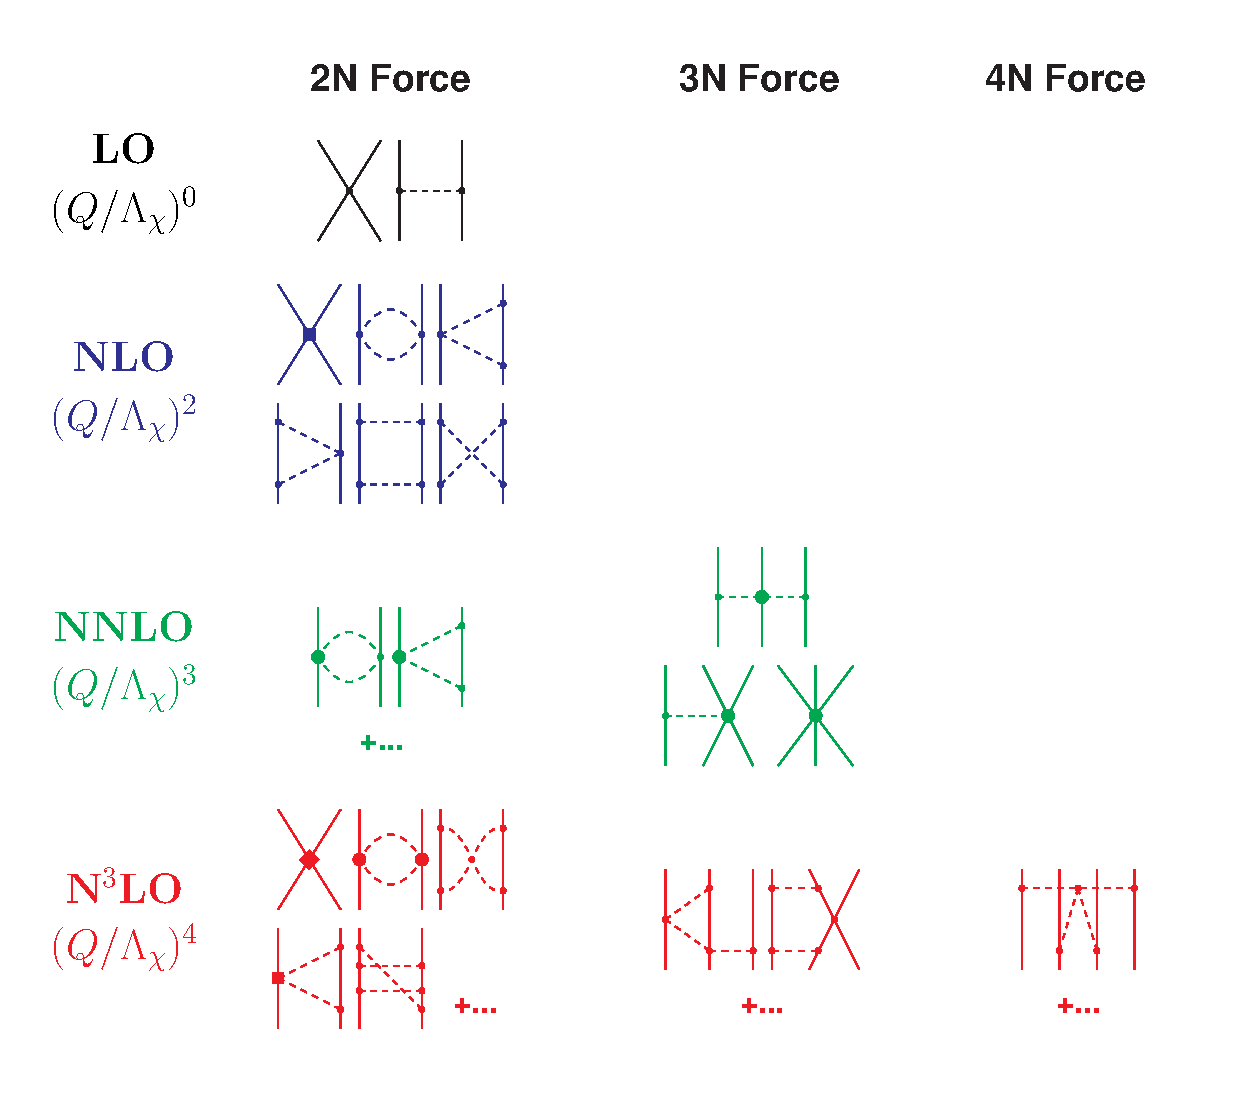
\includegraphics[width=1.25\textwidth]{Figures/diaghi.pdf}
      \end{center}
\column{4.5cm}
\begin{itemize}
\item Nucleons and Pions as effective degrees of freedom only. Most general Lagrangian consistent with all symmetries of low-energy QCD.
\item Chiral perturbation theory for different orders ($\nu$) of the expansion in terms of $(Q/\Lambda_{\chi})^{\nu}$.
\item At order $\nu=4$ one should include four-body forces in many-body calculations!  Not including these will result in what we call missing many-body correlations. 
\end{itemize}
\end{columns}
      \end{footnotesize}
    }


\frame
{
  \frametitle{Forces in Nuclear Physics (without isobars)}
      \begin{figure}[htp]
        \centering	
        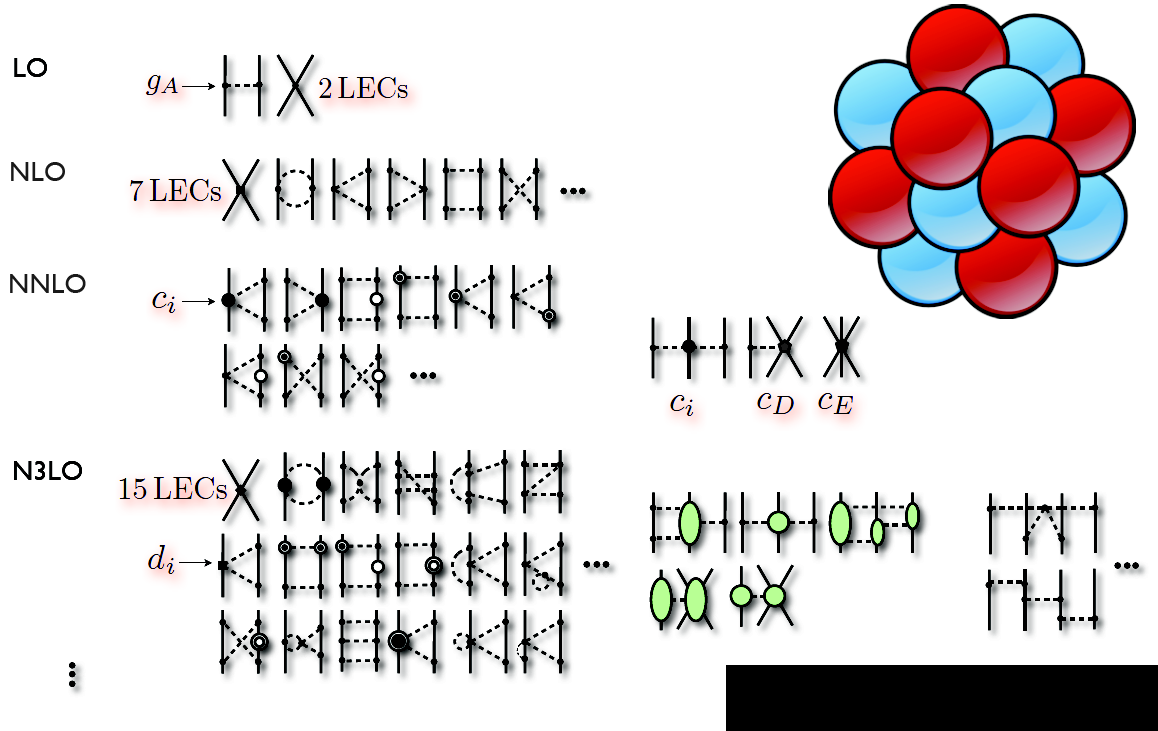
\includegraphics[width=1.0\textwidth]{Figures/forces.png}
      \end{figure}
}







\frame
{
  \frametitle{The future: Hamiltonians from Lattice QCD}
%     \vspace{-3cm}
      \begin{figure}[htp]
        \centering	
        	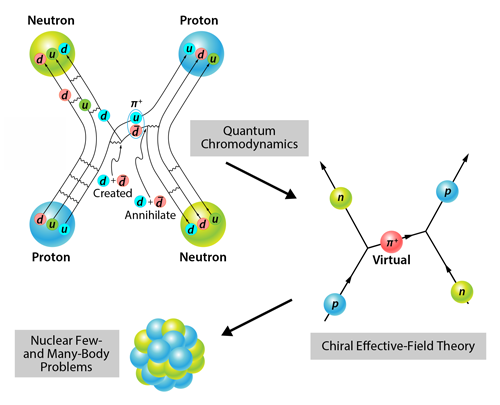
\includegraphics[width=1.0\textwidth]{Figures/future.png}
      \end{figure}
}


\frame
{
  \frametitle{Talent courses in 2019}

\begin{itemize}
\item Nuclear Forces: From Lattice QCD to nuclear effective field theories, approved and to be held at the ECT*, Trento, Italy during  July or August 2019
\item Nuclear Reaction theory, most likely at MSU or University of Ohio during summer 2019
\item New course in China next year!!!
\end{itemize}

{\bf Thanks a million for a fantastic participation. We as teachers have truly enjoyed this time together with you all and it is sad to say that it has to end. You have all been incredible and we hope to see you all again in the near future. Best wishes from all of us and good luck with your thesis work and future projects. }

}





 \end{document}










